\subsubsection{1.3. Quy trình gom cụm và gán nhãn giả lập tự động}

\indent\indent Sau khi trích xuất được các vector biểu diễn của các nút trong đồ thị từ GAE, hệ thống thực hiện quy trình gán nhãn giả lập. Mục tiêu cốt lõi của giai đoạn này là hiện thực hóa hệ thống luật chuyên gia đã đề xuất tại Chương 1 thành một quy trình xử lý dữ liệu tự động, kiến tạo tập dữ liệu có nhãn phục vụ cho các pha huấn luyện có giám sát tiếp theo.\vspace{0.3cm}

Quy trình thực thi tổng quát được minh họa tại \textbf{Hình \ref{fig:ClusterAndPseudoPipeline}}, tập trung vào luồng biến đổi từ vector embedding sang các thực thể có nhãn định danh:

\begin{figure}[H]
    \centering
    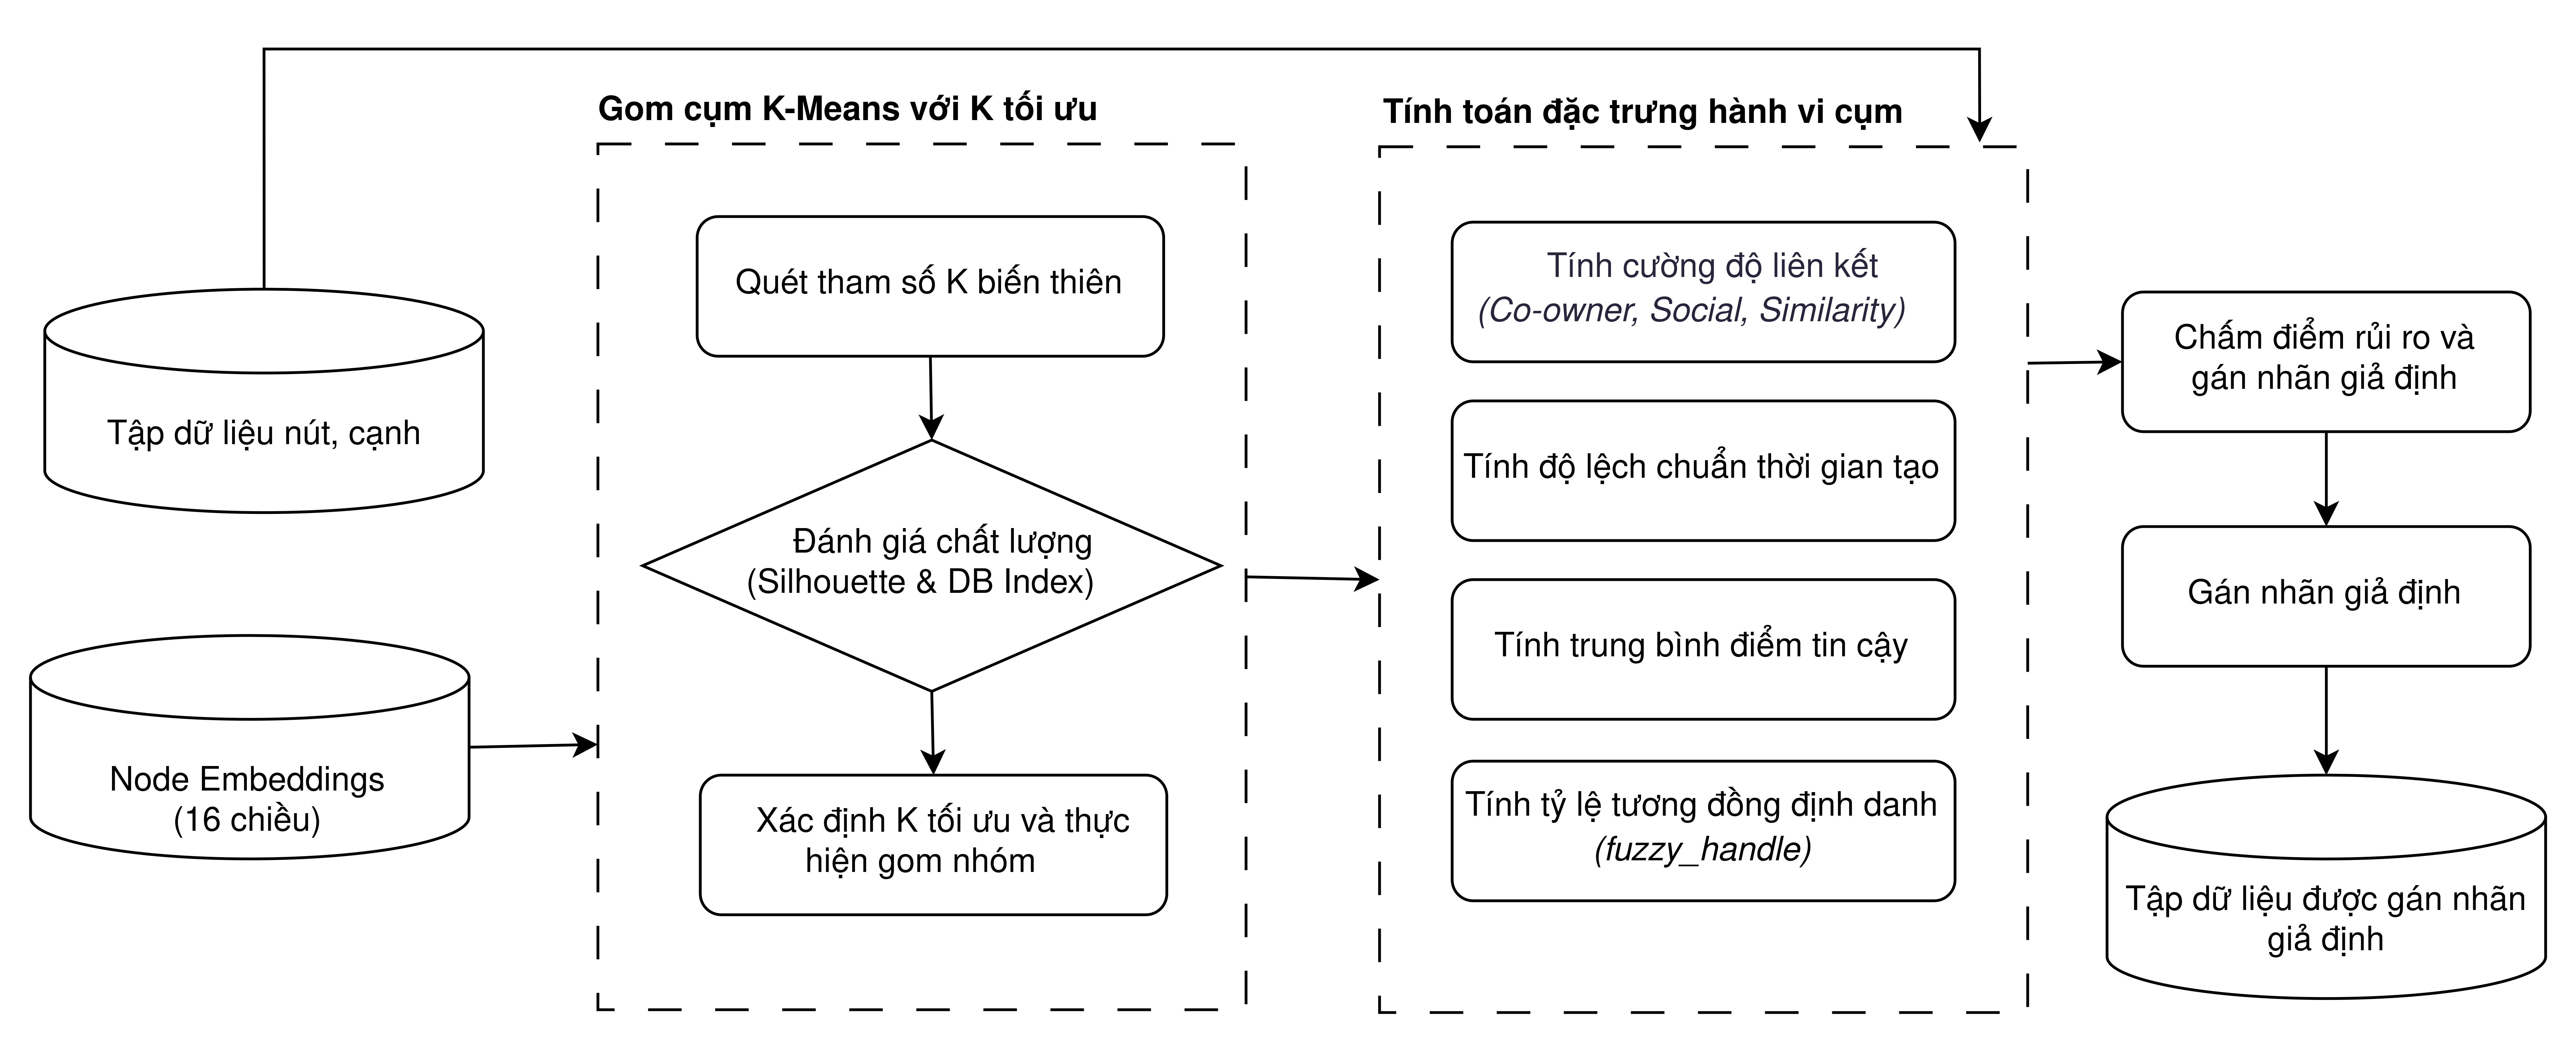
\includegraphics[width=\linewidth]{images/part-02/chap-02/sec-01/ClusterAndPseudoPipeline.png}
    \vspace{0.2cm}
    \caption{Quy trình thực thi gán nhãn giả lập tổng quát}
    \label{fig:ClusterAndPseudoPipeline}
\end{figure}

\textit{1.3.1. Tối ưu hóa phân cụm K-Means}\vspace{0.2cm}

Hệ thống triển khai quy trình tìm kiếm tham số tối ưu tự động thay vì sử dụng một giá trị $K$ cố định nhằm thích ứng với các quy mô dữ liệu theo Tuần, Tháng và Quý. Giá trị $K$ được xác định dựa trên sự hội tụ của hệ số Silhouette và chỉ số Davies-Bouldin, đảm bảo các nhóm hành vi Sybil được cô lập chặt chẽ trong không gian tiềm ẩn trước khi tiến hành định lượng rủi ro.\vspace{0.3cm}

\textit{1.3.2. Hệ thống định lượng rủi ro dựa trên ràng buộc}\vspace{0.2cm}

Tại bước này, hệ thống thực hiện tính toán các chỉ số thống kê đặc trưng cho từng cụm. Dữ liệu từ các cạnh nội bộ của các cụm được lọc và định lượng dựa trên cường độ liên kết và mật độ vi phạm. Chi tiết cơ chế kiểm tra điều kiện song song và tổng hợp điểm rủi ro được minh họa tại \textbf{Hình \ref{fig:ScoringLogic}}.

\begin{figure}[H]
    \centering
    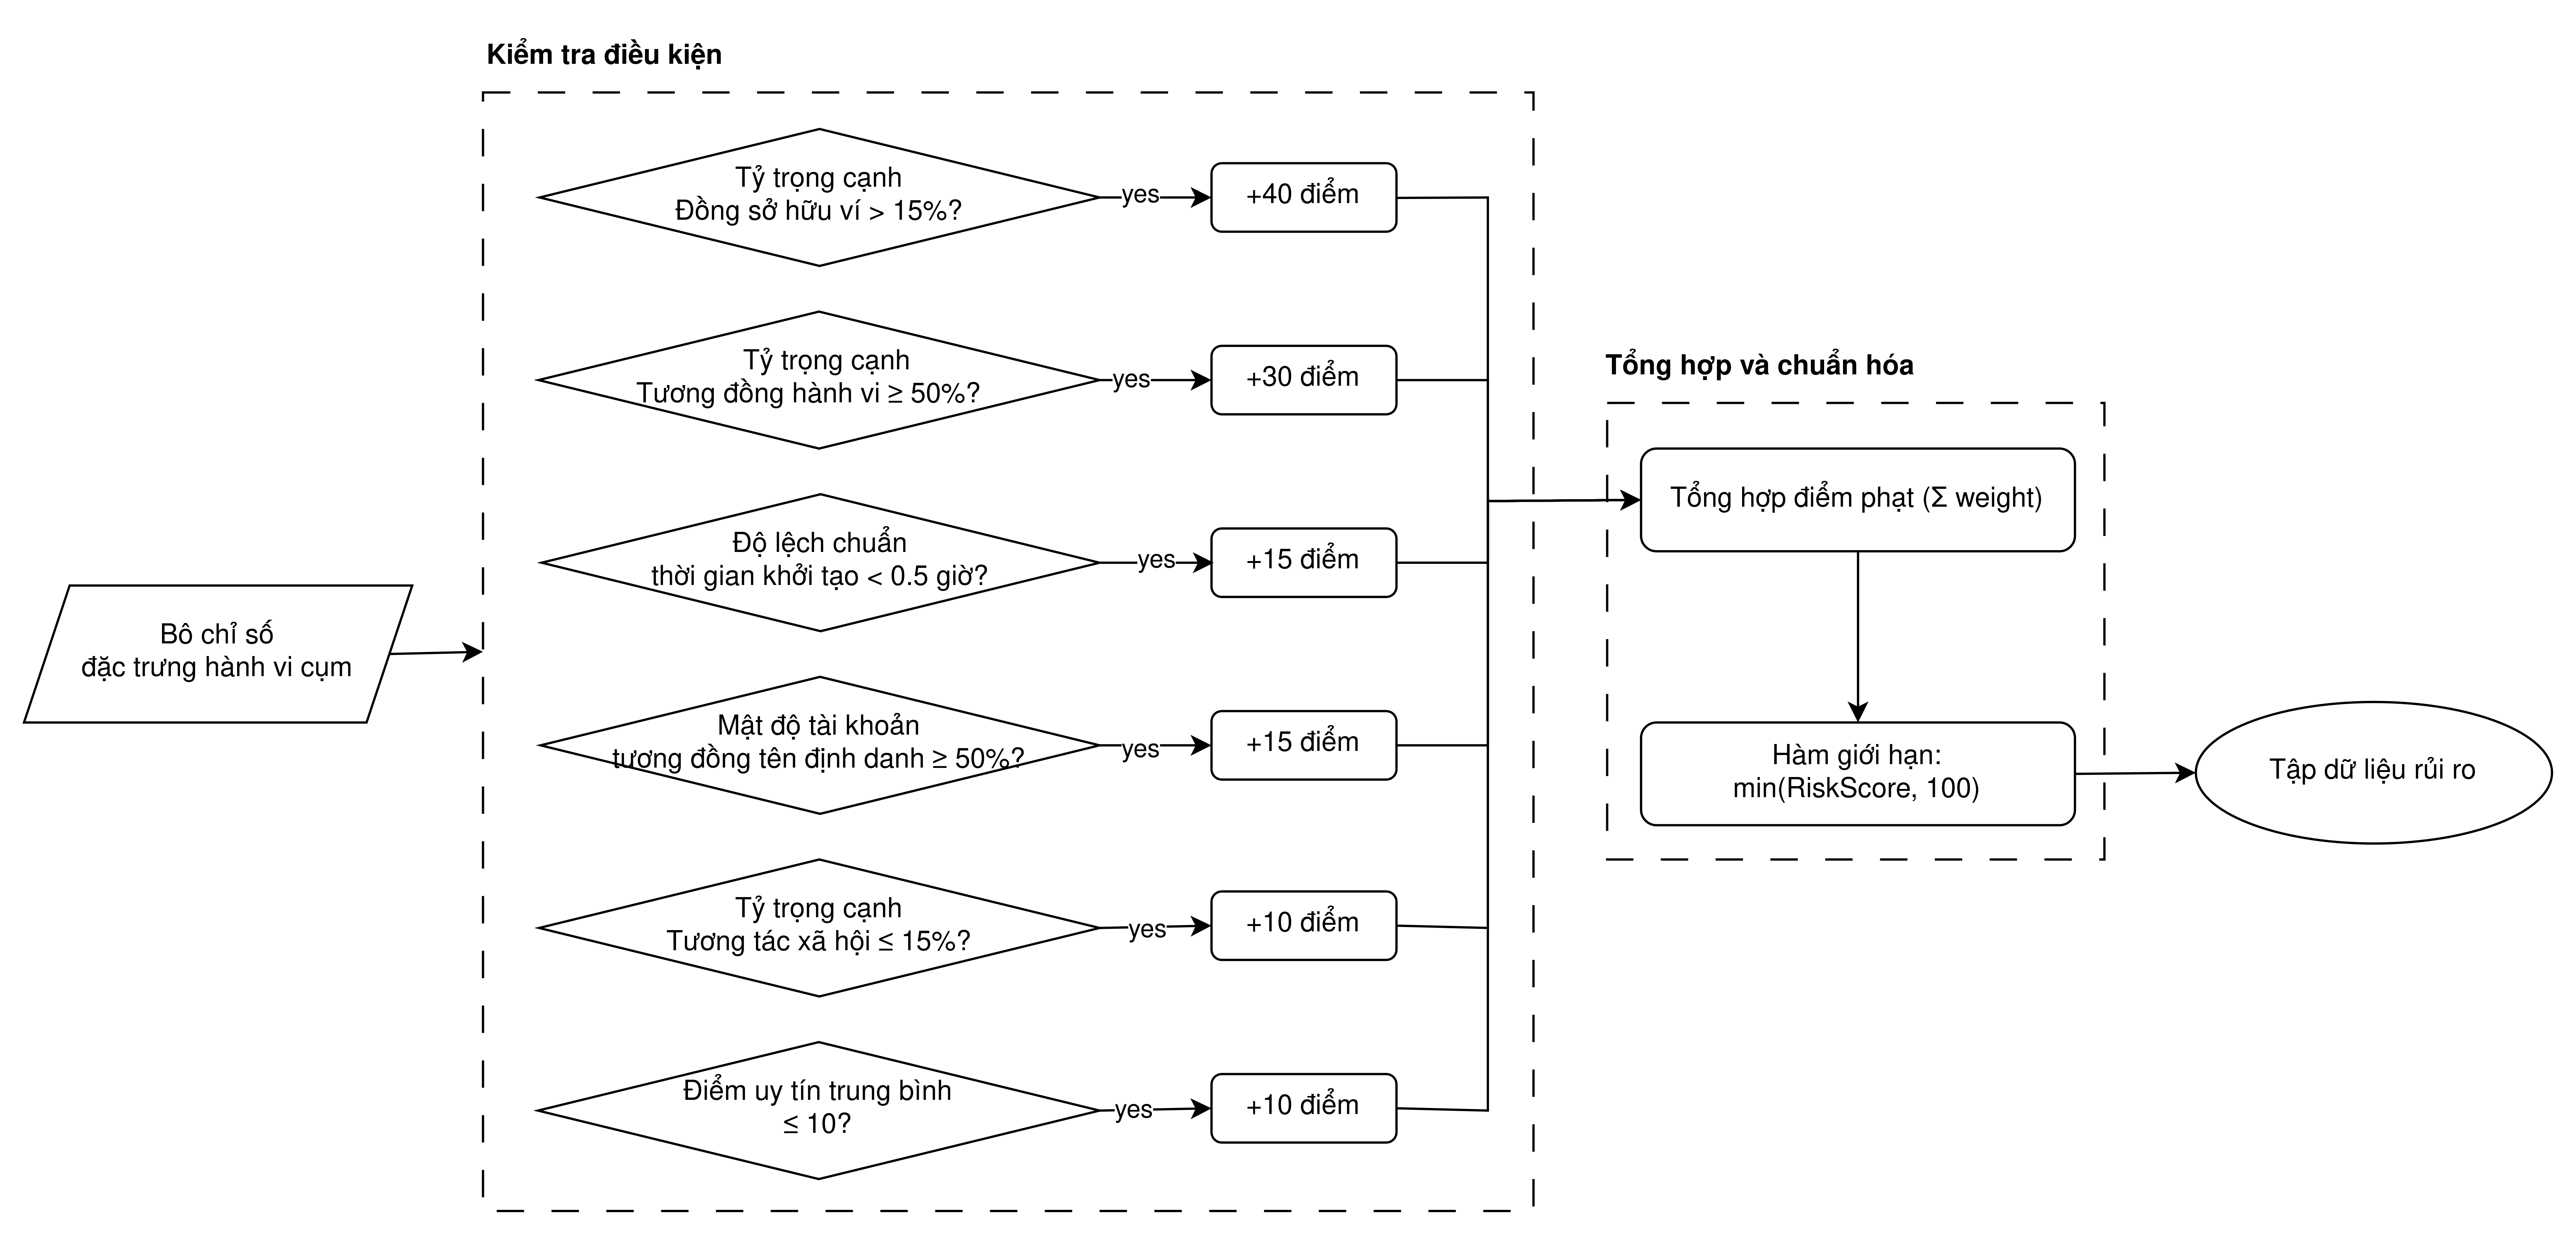
\includegraphics[width=\linewidth]{images/part-02/chap-02/sec-01/Scoring.png}
    \vspace{0.2cm}
    \caption{Cơ chế kiểm tra điều kiện song song và tổng hợp điểm rủi ro}
    \label{fig:ScoringLogic}
\end{figure}

Hệ thống vận hành 6 quy tắc kiểm tra song song, bao gồm việc tính toán tỷ trọng cạnh Đồng sở hữu, Tương đồng hành vi, Tương tác xã hội và điểm uy tín trung bình. Đặc biệt, mật độ vi phạm tương đồng định danh được kiểm tra để tăng độ chính xác trong nhận diện. Tổng điểm rủi ro $S_{risk}$ cuối cùng được chuẩn hóa qua hàm giới hạn $min(Score, 100)$.\vspace{0.3cm}

\textit{1.3.3. Cơ chế phân lớp mờ}\vspace{0.2cm}

Dựa trên tập dữ liệu rủi ro thu được, hệ thống áp dụng kỹ thuật phân lớp mờ (\textit{Fuzzy Labeling}) để ánh xạ điểm số sang 4 cấp độ nhãn rủi ro. Quy trình này được chi tiết hóa tại \textbf{Hình \ref{fig:LabelingLogic}}.

\begin{figure}[H]
    \centering
    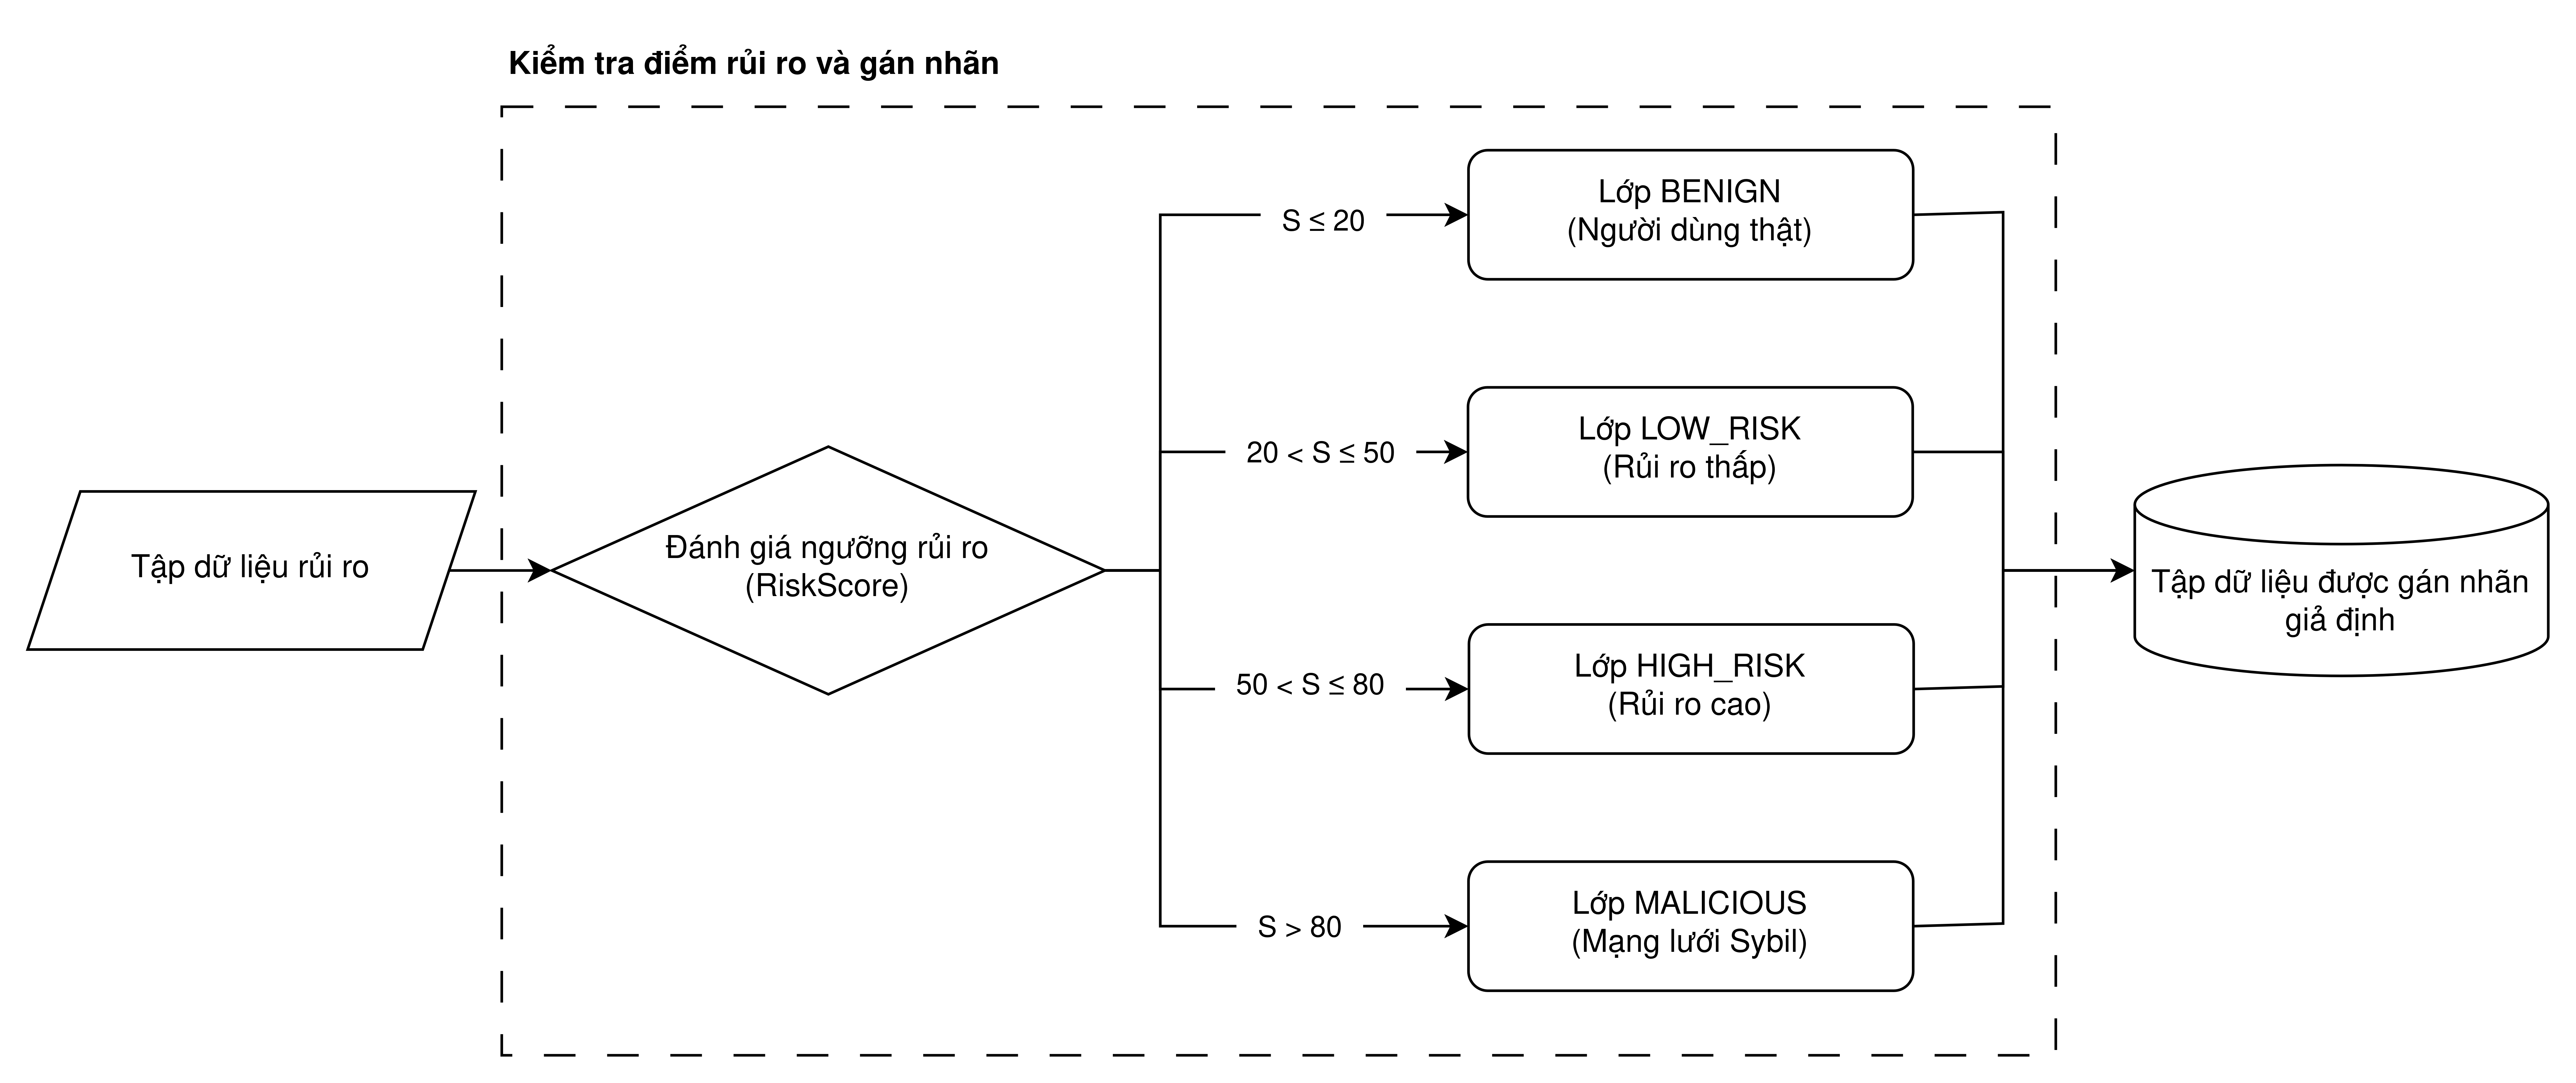
\includegraphics[width=\linewidth]{images/part-02/chap-02/sec-01/Labeling.png}
    \vspace{0.2cm}
    \caption{Cơ chế phân lớp mờ và đồng bộ hóa nhãn nội cụm}
    \label{fig:LabelingLogic}
\end{figure}

Điểm nổi bật của quy trình là tính giải thích, khi mỗi nhãn dán đều được đính kèm các lý do vi phạm thu được từ bước chấm điểm trước đó. Kết quả đầu ra là một tập dữ liệu có cấu trúc hoàn chỉnh, đóng vai trò là tín hiệu giám sát để tối ưu hóa hàm mục tiêu cho các mô hình GNN và kiến trúc Decoupled ML ở các bước tiếp theo.